\chapter{Results Of Testing On Various Cases}
To evaluate the performance of the CPR implementation on \texttt{UTCOMPRS}, four compositional cases were
run. These cases were originaly presented in \cite{fernandes}, in an Adaptive-Implicit study in \texttt{UTCOMPRS}. 
The first case (\texttt{Case 1}) is a three-phase model that involves gas injection and aimed 
at testing the effects of dispersion. The second case (\texttt{Case 2}) is a gas-flooding model in 
a heterogeneous reservoir. The third case (\texttt{Case 3}) is a four-phase $CO_{2}$ flooding model 
in an areal heterogeneous reservoir. The fourth and final case (\texttt{Case 4}) is an extension of
the third case to 3D. These cases are presented below and compared with CPR preconditioner against
the standard solver in \texttt{UTCOMPRS} which is a Krylov based \texttt{GMRES} with \texttt{ILU(0)} as a global
preconditioner. 

\section{Case 1}
The details of the reservoir being simulated are shown in table \ref{case1}. 

\FloatBarrier
\begin{center}
\begin{table}[h!]
\begin{adjustbox}{width=0.8\textwidth}
    \begin{threeparttable}
    \caption{\textbf{Case 1 Reservoir Parameters\supercite{fernandes}.}}
    \label{case1}
        \begin{tabular}{l r }
            \toprule
            Simulatoin Parameters & Value\\
            \midrule
	\rowcolor{red!20}\textit{\textbf{Reservoir data}}      & \\
	Grid:      &           $160\times160\times10$ ($256,000$ active) \\
	\rowcolor{blue!5}Number of wells:      &  2 (1 injector / 1 producer) \\
	Length, width and thickness:      & $170.69$ m, $170.69$ m and $30.48$ m\\
	\rowcolor{blue!5}Porosity:       &          $0.35$ \\
	Initial water saturation:    & $0.3$ \\      
	\rowcolor{blue!5}Initial pressure:    &      $10.34$ MPa\\
	Formation temperature:    & $344.26$ K     \\
	\rowcolor{blue!5}Tortuosity:    &      $1.0$ \\
	Longitudinal dispersivity (W/O/G):    & $4.74$ m, $4.74$ m, and $4.74$ m\\
	\rowcolor{blue!5}Transversal dispersivity (W/O/G):    & $0.474$ m, $0.474$ m, and $0.474$ m\\
	Gas injection rate:    &       $28,316 \ m^{3}/d$ \\
	\rowcolor{blue!5}Producer’s bottom hole pressure:    &       $8.96$ MPa\\
	Reservoir’s initial composition ($C_{1}$, $C_{3}$, $C_{6}$, $C_{10}$, $C_{15}$ and $C_{20}$): & $0.5$, $0.03$, $0.07$, $0.2$, $0.15$, and $0.05$\\
	\rowcolor{blue!5}Injection fluid composition ($C_{1}$, $C_{3}$, $C_{6}$, $C_{10}$, $C_{15}$ and $C_{20}$):    &   $0.77$, $0.2$, $0.01$, $0.01$, $0.005$, and $0.005$\\
	\rowcolor{red!20}\textit{\textbf{Run data}}    &       \\
	Simulation time (days):    &  $1,000$\\
	\rowcolor{blue!5}Simulation time (pore volumes):    & $0.822$\\
            \bottomrule
        \end{tabular}
    \end{threeparttable}
\end{adjustbox}    
\end{table}
\end{center}
\FloatBarrier

\begin{figure}
\centering
\begin{subfigure}{.5\textwidth}
  \centering
  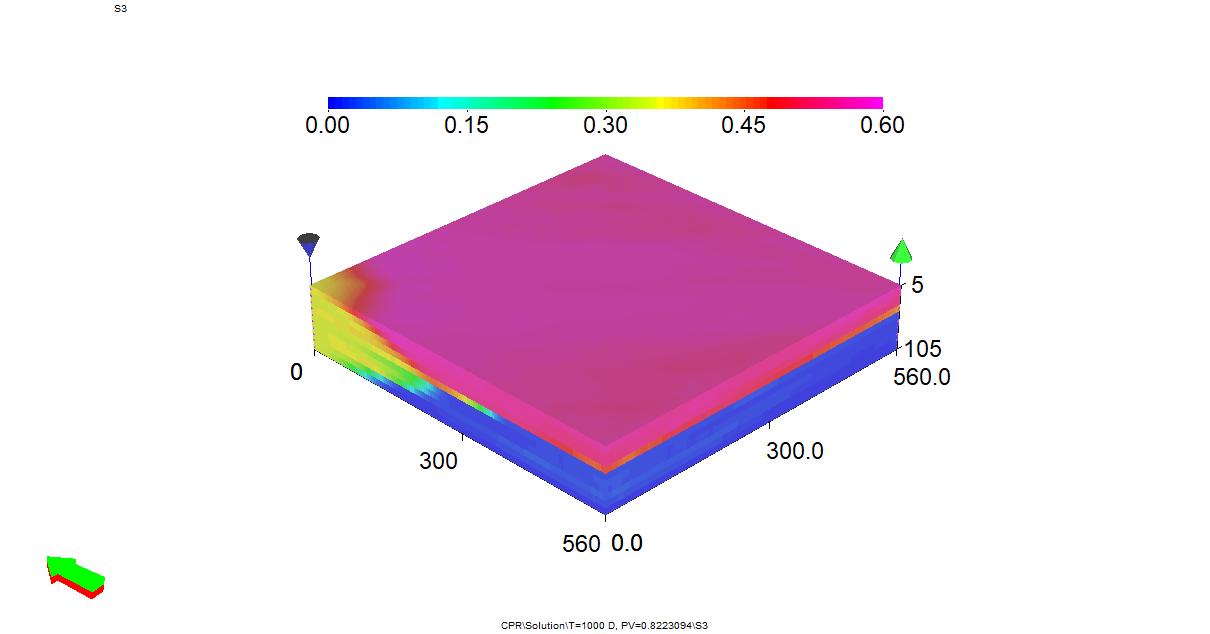
\includegraphics[width=1.3\linewidth]{figures/case1_cpr_sgas.png}
  \caption{\texttt{CPR-AMG} preconditioner.}
\end{subfigure}%
\begin{subfigure}{.5\textwidth}
  \centering
  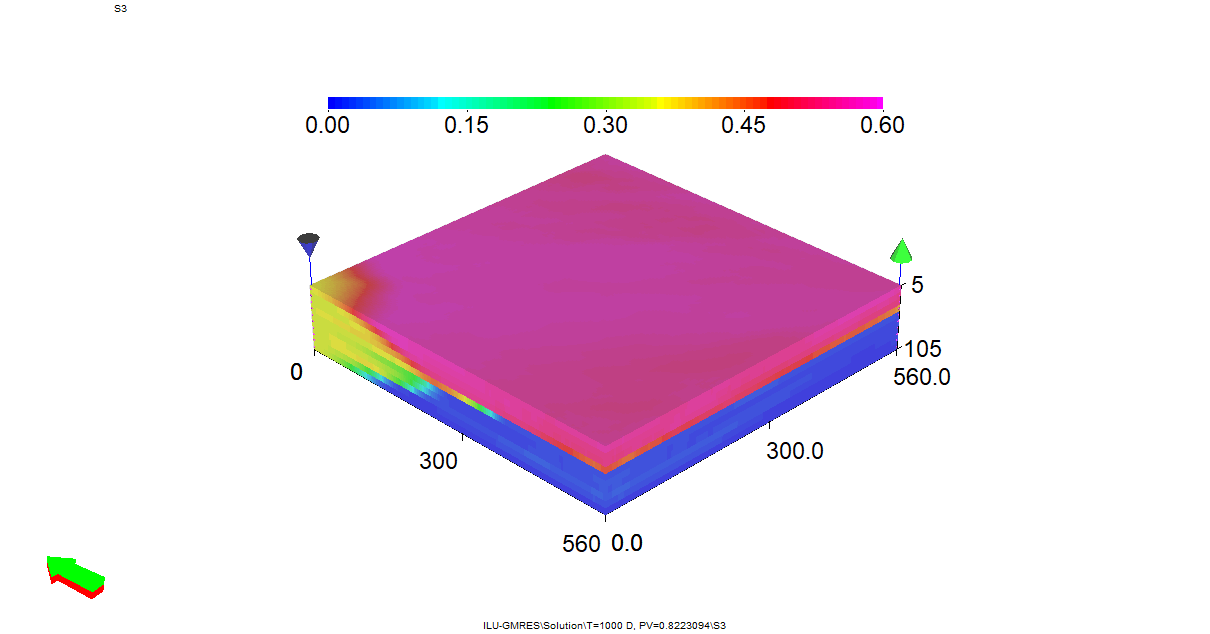
\includegraphics[width=1.3\linewidth]{figures/case1_ilu_sgas.png}
  \caption{\texttt{GMRES-ILU(0)} preconditioner}
\end{subfigure}
\caption{A comparison of \texttt{Case 1} gas saturation $S_{g}$ distribution for the two different preconditioning methods after 1000 days of simulation.}
\label{case1sg}
\end{figure}

\section{Case 2}

\FloatBarrier
\begin{center}
\begin{table}[h!]
\begin{adjustbox}{width=0.8\textwidth}
    \begin{threeparttable}
    \caption{\textbf{Case 2 Reservoir Parameters\supercite{fernandes}.}}
    \label{case1}
        \begin{tabular}{l r }
            \toprule
            Simulatoin Parameters & Value\\
            \midrule
	\rowcolor{red!20}\textit{\textbf{Reservoir data}}      & \\
	Grid:      &           $200\times400\times25$ ($465,816$ active) \\
	\rowcolor{blue!5}Number of wells:      &  49 (25 injectors / 24 producers) \\
	Length, width and thickness:      & $1,219.2$ m, $2,438.4$ m and $45.72$ m\\
	Initial water saturation:    & $0.17$ \\      
	\rowcolor{blue!5}Initial pressure:    &      $20.68$ MPa\\
	Formation temperature:    & $303.15$ K     \\
	Gas injection rate:    &       $86,366 \ m^{3}/d$ \\
	\rowcolor{blue!5}Producer’s bottom hole pressure:    &       $20.68$ MPa\\
	Reservoir’s initial composition ($C_{1}$, $C_{3}$ $C_{10}$): & $0.1$, $0.19$, $0.8$\\
	\rowcolor{blue!5}Injection fluid composition ($C_{1}$, $C_{3}$, $C_{10}$):    &   $0.95$, $0.05$, $0.0$\\
	\rowcolor{red!20}\textit{\textbf{Run data}}    &       \\
	Simulation time (days):    &  $2,190$\\
	\rowcolor{blue!5}Simulation time (pore volumes):    & $1.477$\\
            \bottomrule
        \end{tabular}
    \end{threeparttable}
\end{adjustbox}    
\end{table}
\end{center}
\FloatBarrier

\section{Case 3}

\FloatBarrier
\begin{center}
\begin{table}[h!]
\begin{adjustbox}{width=\textwidth}
    \begin{threeparttable}
    \caption{\textbf{Case 3 Reservoir Parameters\supercite{fernandes}.}}
    \label{case1}
        \begin{tabular}{l r }
            \toprule
            Simulatoin Parameters & Value\\
            \midrule
	\rowcolor{red!20}\textit{\textbf{Reservoir data}}      & \\
	Grid:      &           $200\times200\times10$ ($99,816$ active) \\
	\rowcolor{blue!5}Number of wells:      &  2 (1 injector / 1 producer) \\
	Length, width and thickness:      & $152.4$ m, $304.8$ m and $6.096$ m\\
	\rowcolor{blue!5}Porosity:       &          $0.25$ \\
	Initial water saturation:    & $0.35$ \\      
	\rowcolor{blue!5}Initial pressure:    &      $7.58$ MPa\\
	Formation temperature:    & $313.71$ K     \\
	injector's bottom hole pressure:    &       $8.62$ MPa \\
	\rowcolor{blue!5}Producer’s bottom hole pressure:    &       $7.58$ MPa\\
	Reservoir’s initial composition ($CO_{2}$, $C_{1}$, $C_{2-3}$, $C_{4-6}$, $C_{7-15}$, $C_{16-27}$, $C_{28+}$) & $0.0337$, $0.0861$, $0.1503$, $0.1671$, $0.3304$, $0.1611$ and $0.0713$\\
	\rowcolor{blue!5}Injection fluid composition ($CO_{2}$, $C_{1}$):    &   $0.95$, $0.05$\\
        \bottomrule
        \end{tabular}
    \end{threeparttable}
\end{adjustbox}    
\end{table}
\end{center}
\FloatBarrier

\begin{figure}
\centering
\begin{subfigure}{.5\textwidth}
  \centering
  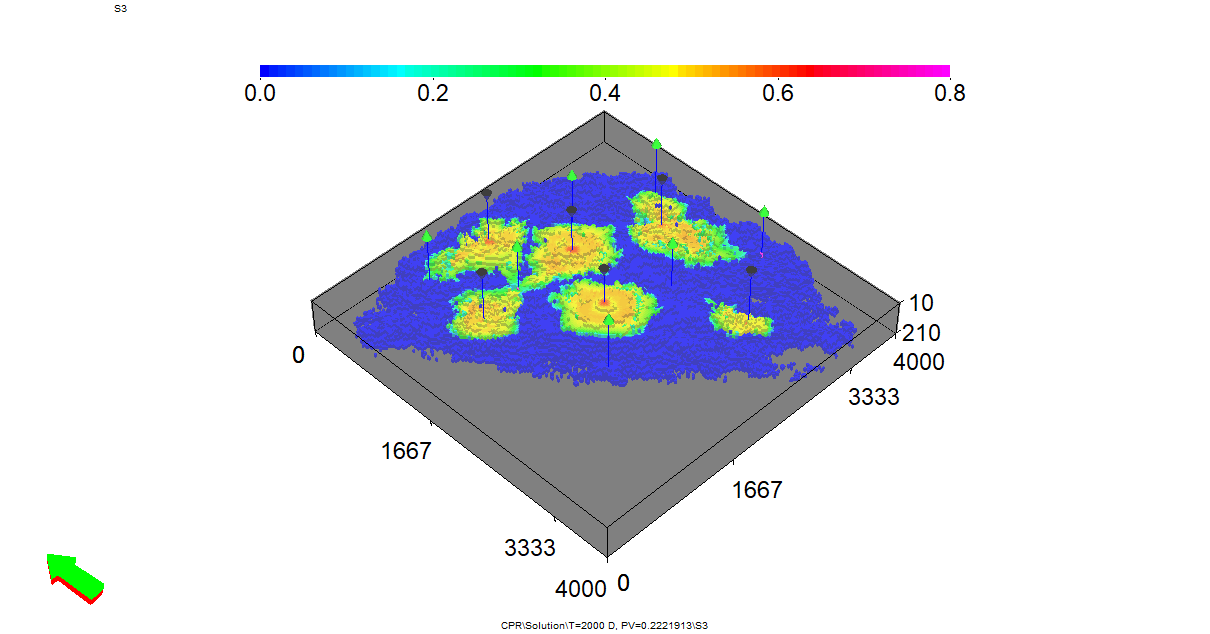
\includegraphics[width=1.3\linewidth]{figures/case3_cpr_sgas.png}
  \caption{\texttt{CPR-AMG} preconditioner.}
\end{subfigure}%
\begin{subfigure}{.5\textwidth}
  \centering
  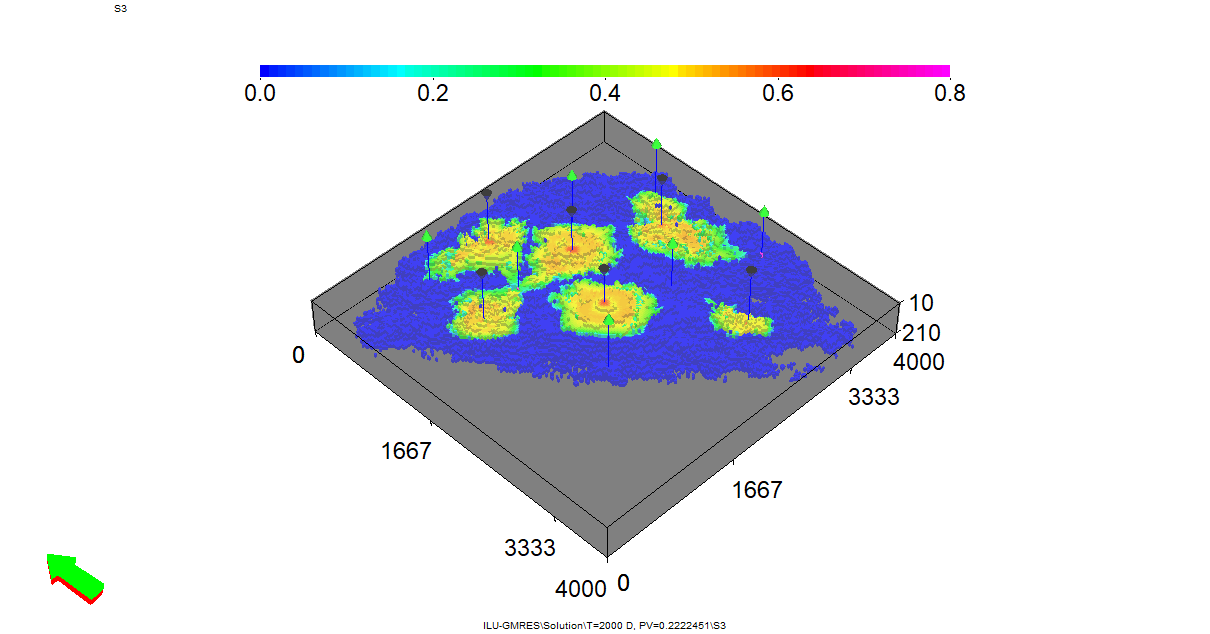
\includegraphics[width=1.3\linewidth]{figures/case3_ilu_sgas.png}
  \caption{\texttt{GMRES-ILU(0)} preconditioner}
\end{subfigure}
\caption{A comparison of \texttt{Case 3} gas saturation $S_{g}$ distribution for the two different preconditioning methods after 2000 days of simulation.}
\label{case1sg}
\end{figure}

\begin{figure}
\centering
\begin{subfigure}{.5\textwidth}
  \centering
  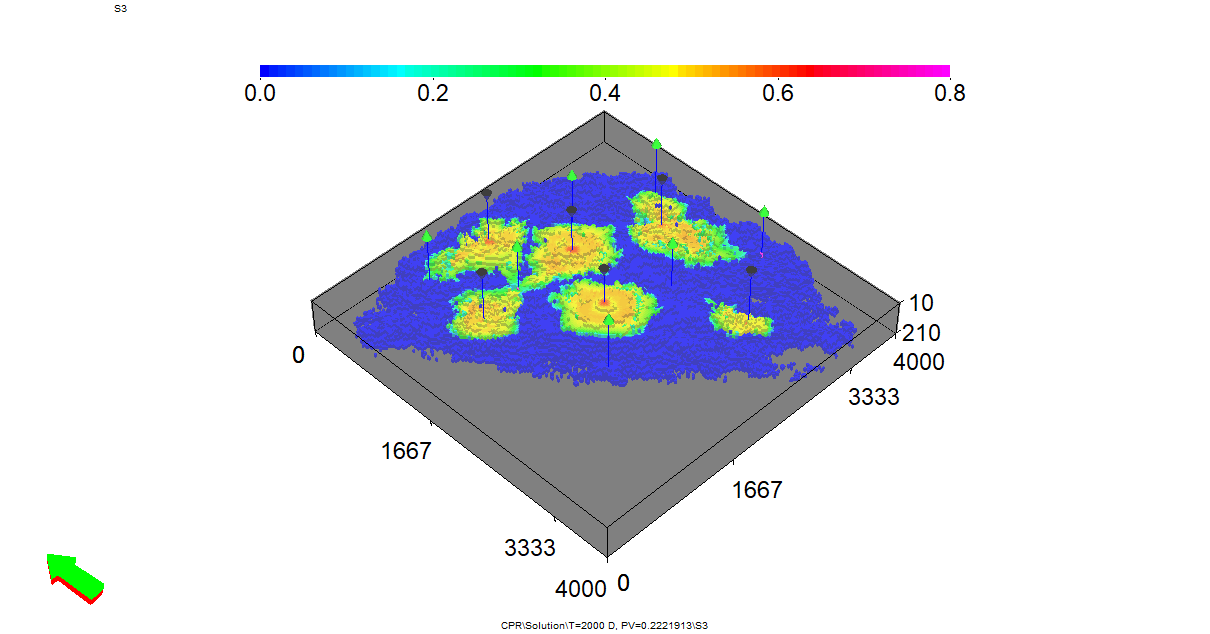
\includegraphics[width=1.3\linewidth]{figures/case3_cpr_sgas.png}
  \caption{\texttt{CPR-AMG} preconditioner.}
\end{subfigure}%
\begin{subfigure}{.5\textwidth}
  \centering
  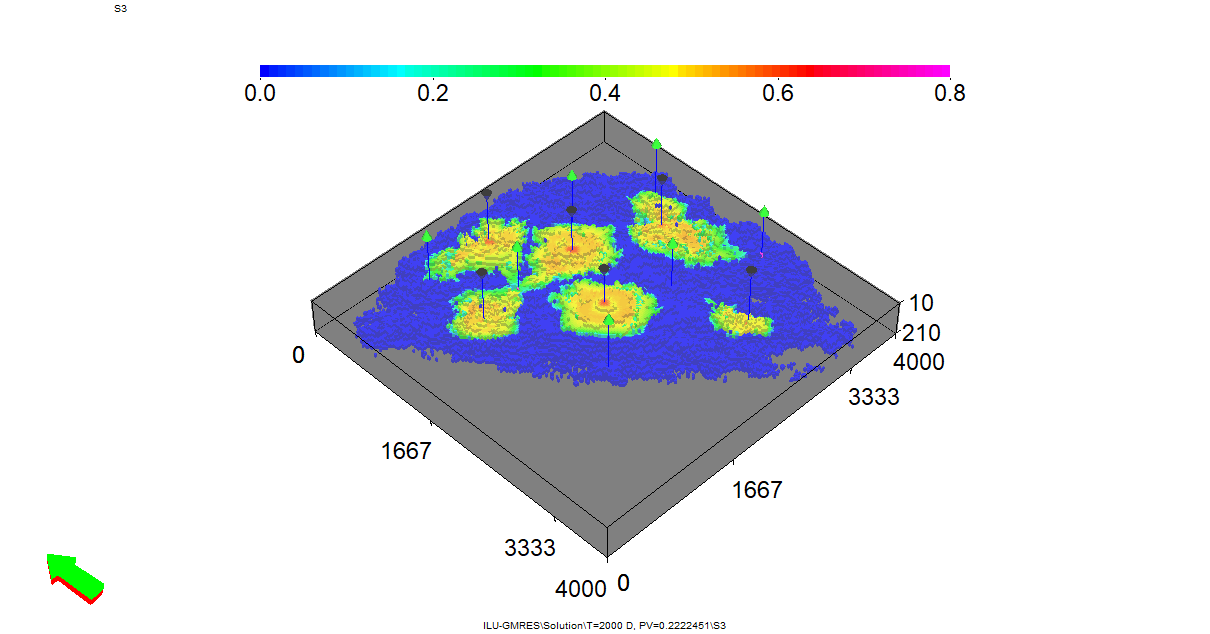
\includegraphics[width=1.3\linewidth]{figures/case3_ilu_sgas.png}
  \caption{\texttt{GMRES-ILU(0)} preconditioner}
\end{subfigure}
\caption{A comparison of \texttt{Case 3} $CO_{2}$ overall composition $Z_{CO_{2}}$ distribution for the two different preconditioning methods after 2000 days of simulation.}
\label{case1sg}
\end{figure}

\section{Case 4}

\FloatBarrier
\begin{center}
\begin{table}[h!]
\begin{adjustbox}{width=\textwidth}
    \begin{threeparttable}
    \caption{\textbf{Case 3 Reservoir Parameters\supercite{fernandes}.}}
    \label{case1}
        \begin{tabular}{l r }
            \toprule
            Simulatoin Parameters & Value\\
            \midrule
	\rowcolor{red!20}\textit{\textbf{Reservoir data}}      & \\
	Grid:      &           $200\times200\times10$ ($99,816$ active) \\
	\rowcolor{blue!5}Number of wells:      &  2 (1 injector / 1 producer) \\
	Length, width and thickness:      & $152.4$ m, $304.8$ m and $6.096$ m\\
	\rowcolor{blue!5}Porosity:       &          $0.25$ \\
	Initial water saturation:    & $0.35$ \\      
	\rowcolor{blue!5}Initial pressure:    &      $7.58$ MPa\\
	Formation temperature:    & $313.71$ K     \\
	injector's bottom hole pressure:    &       $8.62$ MPa \\
	\rowcolor{blue!5}Producer’s bottom hole pressure:    &       $7.58$ MPa\\
	Reservoir’s initial composition ($CO_{2}$, $C_{1}$, $C_{2-3}$, $C_{4-6}$, $C_{7-15}$, $C_{16-27}$, $C_{28+}$) & $0.0337$, $0.0861$, $0.1503$, $0.1671$, $0.3304$, $0.1611$ and $0.0713$\\
	\rowcolor{blue!5}Injection fluid composition ($CO_{2}$, $C_{1}$):    &   $0.95$, $0.05$\\
        \bottomrule
        \end{tabular}
    \end{threeparttable}
\end{adjustbox}    
\end{table}
\end{center}
\FloatBarrier
